\documentclass[11pt]{article}

\usepackage[T1]{fontenc}
\usepackage[utf8]{inputenc}
\usepackage[french]{babel}
\usepackage{amsmath, amssymb, amsthm}
\usepackage{graphicx}
\usepackage{geometry}
\usepackage{enumitem}
\usepackage{hyperref}
\usepackage{mdframed}
\usepackage{mathtools}

\geometry{margin=2.5cm}

% --- Macros utiles ---
\newcommand{\NN}{\mathbb{N}}
\newcommand{\RR}{\mathbb{R}}
\newcommand{\acompleter}{\fbox{À compléter}}

% --- Style des cadres ---
\mdfdefinestyle{coursbox}{
  linewidth=0.8pt,
  linecolor=black,
  backgroundcolor=white,
  roundcorner=0pt,
  innertopmargin=8pt,
  innerbottommargin=8pt,
  innerleftmargin=10pt,
  innerrightmargin=10pt,
  skipabove=10pt,
  skipbelow=10pt
}

% --- Environnements simples ---
\newenvironment{remarque}{\par\smallskip\noindent\textbf{Remarque. \\}\ignorespaces}{\par\smallskip}
\newenvironment{exemple}{\par\smallskip\noindent\textbf{Exemple. \\}\ignorespaces}{\par\smallskip}
\newenvironment{exemples}{\par\smallskip\noindent\textbf{Exemples. \\}\ignorespaces}{\par\smallskip}
\newenvironment{demonstration}{\par\smallskip\noindent\textbf{Démonstration. \\}\ignorespaces}{\par\smallskip}
\newenvironment{historique}{\par\smallskip\noindent\textbf{Historique. \\}\ignorespaces}{\par\smallskip}

% --- Environnements encadrés ---
\newmdenv[style=coursbox]{definition}
\newmdenv[style=coursbox]{propriete}
\newmdenv[style=coursbox]{theoreme}

\begin{document}

\begin{definition}
\begin{center}
    {\Huge\bfseries Suites numériques - 2/2}
\end{center}
\end{definition}

\begin{historique}
Une anecdote relate comment le mathématicien allemand Carl Friedrich Gauss (1777--1855), alors âgé de 10 ans, a fait preuve d'un talent remarquable pour le calcul mental. Voulant occuper ses élèves, le professeur leur demande d'effectuer des additions, plus exactement d'effectuer la somme des nombres de 1 à 100. Après très peu de temps, le jeune Gauss impressionne son professeur en donnant la réponse correcte.

Sa technique consiste à regrouper astucieusement les termes extrêmes deux par deux. Sans le savoir encore, Gauss a découvert la formule permettant de calculer la somme des termes d'une suite arithmétique.

Cette méthode de regroupement intelligent deviendra plus tard un pilier fondamental de l'analyse combinatoire et du calcul algébrique, démontrant la puissance de l'intuition mathématique précoce face aux problèmes complexes.
\end{historique}

\section{Suites arithmétiques}

\subsection{Définition}

\begin{definition}
Une suite est dite \emph{arithmétique} lorsqu'on passe d'un terme au suivant en ajoutant un même nombre.

Autrement dit, une suite $(u_n)$ est dite arithmétique s'il existe un nombre réel $r$ tel que, pour tout entier naturel $n$, on ait
\[
u_{n+1}=u_n+r.
\]
Ce nombre $r$ est appelé \emph{raison} de la suite.
\end{definition}

\begin{remarque}
Pour tout $n\in\NN$, $u_{n+1}-u_n=r$.

Les suites arithmétiques modélisent donc des phénomènes à \emph{variations constantes}.
\end{remarque}

\begin{exemples}
\begin{enumerate}[label=\arabic*.]
    \item Soit la suite $u$ définie par $u_n=2n+3$. On a $u_0=3$, $u_1=5$, $u_2=7$ et $u_3=9$. De manière générale,
    \[
    u_{n+1}-u_n=2(n+1)+3-(2n+3)=2.
    \]
    $u$ est donc une suite arithmétique de raison $2$.
    \item Soit la suite $v$ définie par $v_n=n^2+1$. On a $v_0=1$, $v_1=2$ et $v_2=5$. Or $v_1-v_0=1$ et $v_2-v_1=3$. La suite $v$ n'est donc pas arithmétique.
\end{enumerate}
\end{exemples}

\subsection{Forme explicite du terme général d'une suite arithmétique}

\begin{propriete}
Si $(u_n)$ est une suite arithmétique de raison $r$, alors, pour tout entier naturel $n$,
\[
u_n=u_0+nr.
\]
\end{propriete}

\begin{demonstration}
La suite arithmétique $(u_n)$ de raison $r$ et de premier terme $u_0$ vérifie $u_{n+1}=u_n+r$. En calculant les premiers termes,
\[
u_1=u_0+r,\qquad u_2=u_1+r,\qquad u_3=u_2+r,\quad\ldots,\quad u_n=u_{n-1}+r.
\]
En additionnant membre à membre ces $n$ égalités, on obtient
\[
u_1+u_2+u_3+\cdots+u_n=u_0+u_1+u_2+\cdots+u_{n-1}+nr.
\]
En retranchant aux deux membres les termes identiques, il vient $u_n=u_0+nr$.
\end{demonstration}

\begin{exemples}
Pour chaque suite, calculer le terme de rang 20.
\begin{enumerate}[label=\arabic*.]
    \item Soit $(u_n)$ la suite arithmétique de raison $3$ et de premier terme $u_0=6$.
    \item Soit $(v_n)$ la suite arithmétique de raison $4$ telle que $v_{12}=60$.
    \item Soit $(w_n)$ la suite arithmétique telle que $w_3=18$ et $w_{17}=-10$.
\end{enumerate}
\begin{enumerate}[label=\arabic*.]
    \item $u_{20}=u_0+20\times 3=66$.
    \item $v_{20}=v_{12}+8\times 4=92$.
    \item $w_{20}=w_{17}+3r$, avec
    \[
    r=\frac{w_{17}-w_3}{17-3}=-2,
    \]
    d'où $w_{20}=-16$.
\end{enumerate}
\end{exemples}

\subsection{Sens de variation d'une suite arithmétique}

\begin{propriete}
La représentation graphique d'une suite arithmétique est un ensemble de points alignés.

La raison de la suite arithmétique correspond au coefficient directeur de la droite passant par l'ensemble des points représentant la suite, et l'ordonnée à l'origine au terme de rang $0$ de la suite.
\end{propriete}

\begin{exemple}
On a représenté ci-dessous la suite arithmétique de raison $-0{,}5$ et de premier terme $4$ :
\begin{center}
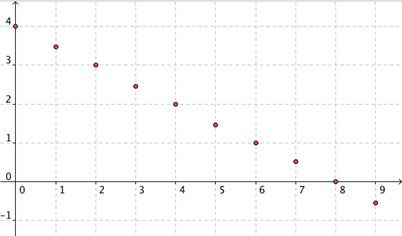
\includegraphics[width=0.4\textwidth]{images/suites_2.png}
\end{center}
\end{exemple}

\begin{propriete}
Soit $u$ une suite arithmétique de raison $r$.
\begin{itemize}
    \item Si $r<0$, la suite arithmétique est strictement décroissante.
    \item Si $r=0$, la suite arithmétique est constante.
    \item Si $r>0$, la suite arithmétique est strictement croissante.
\end{itemize}
\end{propriete}

\begin{demonstration}
Pour tout entier naturel $n$, $u_{n+1}=u_n+r$. Ainsi :
\begin{itemize}
    \item si $r<0$, alors $u_n+r<u_n$, soit $u_{n+1}<u_n$ ; la suite $(u_n)$ est donc strictement décroissante ;
    \item si $r>0$, alors $u_n+r>u_n$, soit $u_{n+1}>u_n$ ; la suite $(u_n)$ est donc strictement croissante.
\end{itemize}
\end{demonstration}

\begin{exemples}
Avec les notations des exemples précédents, les suites $(u_n)$ de raison $3$ et $(v_n)$ de raison $4$ sont strictement croissantes, et la suite $(w_n)$ de raison $-2$ est strictement décroissante.
\end{exemples}

\subsection{Somme des $n$ premiers termes d'une suite arithmétique}

\begin{propriete}
Pour tout entier naturel $n\geq 1$, la somme des $n$ premiers entiers est
\[
S=1+2+3+\cdots+n=\frac{n(n+1)}{2}.
\]
\end{propriete}

\begin{demonstration}
Notons $S=1+2+3+\cdots+n$. On effectue cette somme dans les deux sens :
\begin{align*}
S&=1+2+3+\cdots+n,\\
S&=n+(n-1)+(n-2)+\cdots+1,\\
2S&=(n+1)+(n+1)+(n+1)+\cdots+(n+1).
\end{align*}
On en déduit que $2S=n(n+1)$, d'où
\[
S=\frac{n(n+1)}{2}.
\]
\end{demonstration}

\begin{propriete}
Soit $u$ une suite arithmétique de raison $r$ et de premier terme $u_0$. Pour tout entier naturel $n\geq 1$, la somme des $n$ premiers termes de la suite est
\[
S=u_0+u_1+u_2+\cdots+u_{n-1}=n\,\frac{u_0+u_{n-1}}{2}.
\]
\end{propriete}

\begin{demonstration}
Pour tout entier $k$, $u_k=u_0+kr$. Donc
\begin{align*}
S&=u_0+u_1+u_2+\cdots+u_{n-1}\\
 &=u_0+(u_0+r)+(u_0+2r)+\cdots+(u_0+(n-1)r)\\
 &=nu_0+r(1+2+3+\cdots+(n-1))\\
 &=nu_0+r\frac{n(n-1)}{2}\\
 &=n\left(u_0+\frac{r(n-1)}{2}\right)\\
 &=n\,\frac{u_0+u_0+r(n-1)}{2}\\
 &=n\,\frac{u_0+u_{n-1}}{2}.
\end{align*}
\end{demonstration}

\begin{theoreme}
La somme des termes consécutifs d'une suite arithmétique est la moyenne arithmétique des termes extrêmes multipliée par le nombre de termes sommés :
\[
S=\text{nombre de termes sommés}\times
\frac{\text{premier terme sommé}+\text{dernier terme sommé}}{2}.
\]
\end{theoreme}

\begin{exemples}
\begin{enumerate}[label=\arabic*.]
    \item Somme des multiples de $3$ entre $12$ et $27$.
    \item Somme des $n$ premiers entiers impairs.
\end{enumerate}
\begin{enumerate}[label=\arabic*.]
    \item La suite des multiples positifs de $3$ est arithmétique de raison $3$ et de premier terme $3$ : $3,6,9,\ldots$. Il y a $6$ multiples de $3$ entre $12$ et $27$, donc leur somme vaut
    \[
    6\times\frac{12+27}{2}=117.
    \]
    \item La suite des entiers impairs est la suite $u$ de terme général $u_n=2n+1$. Elle est arithmétique de raison $2$ et de premier terme $u_0=1$. On a donc
    \begin{align*}
    1+3+5+\cdots+2(n-1)+1
      &=u_0+u_1+u_2+\cdots+u_{n-1}\\
      &=n\,\frac{u_0+u_{n-1}}{2}\\
      &=n\,\frac{1+2(n-1)+1}{2}=n^2.
    \end{align*}
\end{enumerate}
\end{exemples}

\section{Suites géométriques}

\subsection{Définition}

\begin{definition}
Une suite est dite \emph{géométrique} lorsqu'on passe d'un terme au suivant en multipliant par un nombre constant.

Autrement dit, une suite $(u_n)$ est dite géométrique s'il existe un nombre réel $q$ non nul tel que, pour tout entier naturel $n$, on ait
\[
u_{n+1}=q\,u_n.
\]
Ce nombre $q$ est encore appelé \emph{raison} de la suite.
\end{definition}

\begin{remarque}
Pour tout $n\in\NN$, si $u_n\neq 0$, on a $\dfrac{u_{n+1}}{u_n}=q$.

Les suites géométriques modélisent donc des phénomènes à \emph{variations relatives constantes}.
\end{remarque}

\begin{exemples}
\begin{enumerate}[label=\arabic*.]
    \item Soit la suite $u$ définie par $u_n=2^n$. On a $u_0=1$, $u_1=2$, $u_2=4$ et $u_3=8$. De manière générale,
    \[
    \frac{u_{n+1}}{u_n}=\frac{2^{n+1}}{2^n}=2.
    \]
    $u$ est donc une suite géométrique de raison $2$.
    \item Soit la suite $v$ définie par $v_n=n^2+1$. On a $v_0=1$, $v_1=2$ et $v_2=5$. Or $\dfrac{v_1}{v_0}=\dfrac21=2$ et $\dfrac{v_2}{v_1}=\dfrac52$. La suite $v$ n'est donc pas géométrique.
\end{enumerate}
\end{exemples}

\subsection{Forme explicite du terme général d'une suite géométrique}

\begin{propriete}
Si $(u_n)$ est une suite géométrique de raison $q$, alors, pour tout entier naturel $n$,
\[
u_n=u_0q^n.
\]
\end{propriete}

\begin{demonstration}
La suite géométrique $(u_n)$ de raison $q$ et de premier terme $u_0$ vérifie $u_{n+1}=q\,u_n$.
\begin{itemize}
    \item Si $q$ ou $u_0$ est nul, alors tous les termes de la suite sont nuls. La démonstration est évidente dans ce cas.
    \item Sinon, tous les termes de la suite sont non nuls, et les premiers termes vérifient
    \[
    u_1=qu_0,\qquad u_2=qu_1,\qquad u_3=qu_2,\quad\ldots,\quad u_n=qu_{n-1}.
    \]
    En multipliant membre à membre ces $n$ égalités, on obtient
    \[
    u_1u_2u_3\cdots u_n=u_0u_1u_2\cdots u_{n-1}q^n.
    \]
    Comme les termes de la suite sont non nuls, on peut diviser les deux membres par les facteurs identiques : $u_n=u_0q^n$.
\end{itemize}
\end{demonstration}

\begin{exemples}
Pour chaque suite, calculer le terme de rang $5$.
\begin{enumerate}[label=\arabic*.]
    \item Soit $(u_n)$ la suite géométrique de raison $3$ et de premier terme $u_0=2$.
    \item Soit $(v_n)$ la suite géométrique de raison $5$ telle que $v_2=2$.
    \item Soit $(w_n)$ la suite géométrique à termes positifs telle que $w_2=\dfrac12$ et $w_4=\dfrac18$.
\end{enumerate}
\begin{enumerate}[label=\arabic*.]
    \item $u_5=u_0\times 3^5=486$.
    \item $v_5=v_2\times 5^3=250$.
    \item Pour passer de $w_2$ à $w_4$, on a multiplié $w_2$ par $q^2$, donc
    \[
    q=\sqrt{\frac{w_4}{w_2}}=\frac12.
    \]
    D'où $w_5=w_4\times\dfrac12=\dfrac1{16}$.
\end{enumerate}
\end{exemples}

\subsection{Sens de variation d'une suite géométrique de terme initial positif}

Les termes d'une suite géométrique sont obtenus en appliquant successivement un coefficient multiplicateur (la raison) constant. On parle alors d'\emph{évolution exponentielle}.

\begin{propriete}
Soit $u$ une suite géométrique de terme initial $u_0$ non nul et de raison $q$.
\begin{itemize}
    \item Si $q=1$, la suite est constante.
    \item Si $q>1$ :
    \begin{itemize}
        \item si $u_0>0$, la suite est strictement croissante ;
        \item si $u_0<0$, la suite est strictement décroissante.
    \end{itemize}
    \item Si $0<q<1$ :
    \begin{itemize}
        \item si $u_0>0$, la suite est strictement décroissante ;
        \item si $u_0<0$, la suite est strictement croissante.
    \end{itemize}
\end{itemize}
\end{propriete}

\begin{demonstration}
(Pour le cas $u_0>0$.) Pour tout entier naturel $n$, $u_{n+1}=u_nq$. Donc :
\begin{itemize}
    \item si $0<q<1$, alors $0<u_nq<u_n$, soit $u_{n+1}<u_n$ ; la suite $(u_n)$ est strictement décroissante ;
    \item si $q>1$, alors $u_nq>u_n$, soit $u_{n+1}>u_n$ ; la suite $(u_n)$ est strictement croissante.
\end{itemize}
\end{demonstration}

\begin{exemples}
Avec les notations des exemples précédents, les suites géométriques $(u_n)$ de raison $3$ et $(v_n)$ de raison $5$ sont strictement croissantes, et la suite géométrique $(w_n)$ de raison $\dfrac12$ est strictement décroissante.

On a représenté ci-dessous la suite géométrique de raison $2$ et de premier terme $-4$ :
\begin{center}
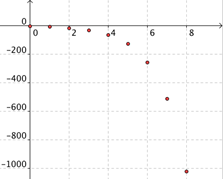
\includegraphics[width=0.3\textwidth]{images/suites_3.png}
\end{center}
\end{exemples}

\subsection{Somme des $n$ premiers termes d'une suite géométrique}

\begin{propriete}
Pour tout nombre réel $q$ différent de $1$, la somme des $n$ premières puissances de $q$ est
\[
S=q^0+q^1+q^2+\cdots+q^{n-1}=\frac{1-q^n}{1-q}.
\]
\end{propriete}

\begin{demonstration}
Posons $S=1+q+q^2+\cdots+q^{n-1}$. Alors
\[
qS=q+q^2+q^3+\cdots+q^n.
\]
Donc
\[
S-qS=1+q+q^2+\cdots+q^{n-1}-(q+q^2+q^3+\cdots+q^n)=1-q^n.
\]
Comme $S-qS=(1-q)S$ et $q\neq 1$, il vient
\[
S=\frac{1-q^n}{1-q}.
\]
\end{demonstration}

\begin{propriete}
Soit $u$ une suite géométrique de raison $q\neq 1$ et de premier terme $u_0$. Pour tout entier naturel $n\geq 1$, la somme des $n$ premiers termes de la suite est
\[
S=u_0+u_1+u_2+\cdots+u_{n-1}=u_0\,\frac{1-q^n}{1-q}.
\]
\end{propriete}

\begin{demonstration}
Pour tout entier $k$, $u_k=u_0q^k$. Donc
\begin{align*}
u_0+u_1+u_2+\cdots+u_{n-1}
 &=u_0q^0+u_0q^1+u_0q^2+\cdots+u_0q^{n-1}\\
 &=u_0(q^0+q^1+q^2+\cdots+q^{n-1})\\
 &=u_0\,\frac{1-q^n}{1-q}.
\end{align*}
\end{demonstration}

\begin{theoreme}
La somme des termes consécutifs d'une suite géométrique est
\[
S=\text{premier terme sommé}\times
\frac{1-\text{raison}^{\text{nombre de termes}}}{1-\text{raison}}.
\]
\end{theoreme}

\begin{exemple}
Calculer la somme des $14$ premiers termes de la suite géométrique $u$ de raison $3$ et de premier terme $u_0=2$.
\[
\begin{aligned}
S&=2+2\times3+2\times3^2+\cdots+2\times3^{13}\\
 &=2\times\frac{1-3^{14}}{1-3}=4\,782\,968.
\end{aligned}
\]
\end{exemple}

\end{document}
